%% Commands for TeXCount
%TC:macro \cite [option:text,text]
%TC:macro \citep [option:text,text]
%TC:macro \citet [option:text,text]
%TC:envir table 0 1
%TC:envir table* 0 1
%TC:envir tabular [ignore] word
%TC:envir displaymath 0 word
%TC:envir math 0 word
%TC:envir comment 0 0

%%
%%
%% The first command in your LaTeX source must be the \documentclass
%% command.
%%
%% For submission and review of your manuscript please change the
%% command to \documentclass[manuscript, screen, review]{acmart}.
%%
%% When submitting camera ready or to TAPS, please change the command
%% to \documentclass[sigconf]{acmart} or whichever template is required
%% for your publication.
%%
%%

% \documentclass[manuscript]{acmart}
\documentclass[sigconf]{acmart}
% \setcopyright{none}
% \documentclass[manuscript]{acmart}

%%
%% \BibTeX command to typeset BibTeX logo in the docs
\AtBeginDocument{\providecommand\BibTeX{{Bib\TeX}}}

%% Rights management information.  This information is sent to you
%% when you complete the rights form.  These commands have SAMPLE
%% values in them; it is your responsibility as an author to replace
%% the commands and values with those provided to you when you
%% complete the rights form.
% \setcopyright{acmcopyright}
% \copyrightyear{2023}
% \acmYear{2023}
% \acmDOI{XXXXXXX.XXXXXXX}

%% These commands are for a PROCEEDINGS abstract or paper.
% \acmConference[Conference acronym 'XX]{Make sure to enter the correct
%   conference title from your rights confirmation emai}{June 03--05,
%   % 2018}{Woodstock, NY}
%%
%%  Uncomment \acmBooktitle if the title of the proceedings is different
%%  from ``Proceedings of ...''!
%%
%%\acmBooktitle{Woodstock '18: ACM Symposium on Neural Gaze Detection,
%%  June 03--05, 2018, Woodstock, NY}
% \acmPrice{15.00}
% \acmISBN{978-1-4503-XXXX-X/18/06}


%%
%% Submission ID.
%% Use this when submitting an article to a sponsored event. You'll
%% receive a unique submission ID from the organizers
%% of the event, and this ID should be used as the parameter to this command.
%%\acmSubmissionID{123-A56-BU3}

%%
%% For managing citations, it is recommended to use bibliography
%% files in BibTeX format.
%%
%% You can then either use BibTeX with the ACM-Reference-Format style,
%% or BibLaTeX with the acmnumeric or acmauthoryear sytles, that include
%% support for advanced citation of software artefact from the
%% biblatex-software package, also separately available on CTAN.
%%
%% Look at the sample-*-biblatex.tex files for templates showcasing
%% the biblatex styles.
%%

%%
%% The majority of ACM publications use numbered citations and
%% references.  The command \citestyle{authoryear} switches to the
%% "author year" style.
%%
%% If you are preparing content for an event
%% sponsored by ACM SIGGRAPH, you must use the "author year" style of
%% citations and references.
%% Uncommenting
%% the next command will enable that style.
%%\citestyle{acmauthoryear}


%%
%% end of the preamble, start of the body of the document source.

% \acmConference[IMX 2023]{ACM International Conference on Interactive Media Experiences}{June 12--15, 2023}{Nantes, France}

\copyrightyear{2023} 
\acmYear{2023} 
\setcopyright{rightsretained} 
\acmConference[IMX '23]{ACM International Conference on Interactive Media Experiences}{June 12--15, 2023}{Nantes, France}
\acmBooktitle{ACM International Conference on Interactive Media Experiences (IMX '23), June 12--15, 2023, Nantes, France}
\acmDOI{10.1145/3573381.3596471}
\acmISBN{979-8-4007-0028-6/23/06}

\begin{document}

%%
%% The "title" command has an optional parameter,
%% allowing the author to define a "short title" to be used in page headers.
\title{Developing an Interactive Agent for Blind and Visually Impaired People}

%%
%% The "author" command and its associated commands are used to define
%% the authors and their affiliations.
%% Of note is the shared affiliation of the first two authors, and the
%% "authornote" and "authornotemark" commands
%% used to denote shared contribution to the research.
\author{Vincent Stragier}
% \authornote{}
\orcid{0000-0002-5850-9817}
\email{vincent.stragier@umons.ac.be}

\affiliation{%
  \institution{Numediart Institute, ISIA Lab, Faculty of Engineering, University of Mons, Mons}
  \streetaddress{Boulevard Dolez, 31}
  \city{Mons}
  \state{Hainaut}
  \country{Belgium}
  \postcode{7000}
}
% \author{}
% \authornotemark[1]
% \email{}

\author{Omar Seddati}
% \authornote{}
\orcid{0000-0002-0573-8480}
\email{omar.seddati@umons.ac.be}

\affiliation{%
  \institution{Numediart Institute, ISIA Lab, Faculty of Engineering, University of Mons, Mons}
  \streetaddress{Boulevard Dolez, 31}
  \city{Mons}
  \state{Hainaut}
  \country{Belgium}
  \postcode{7000}
}


\author{Thierry Dutoit}
% \authornote{}
\orcid{0000-0001-7024-2150}
\email{thierry.dutoit@umons.ac.be}


\affiliation{%
  \institution{Numediart Institute, ISIA Lab, Faculty of Engineering, University of Mons, Mons}
  \streetaddress{Boulevard Dolez, 31}
  \city{Mons}
  \state{Hainaut}
  \country{Belgium}
  \postcode{7000}
}

%%
%% By default, the full list of authors will be used in the page
%% headers. Often, this list is too long, and will overlap
%% other information printed in the page headers. This command allows
%% the author to define a more concise list
%% of authors' names for this purpose.
\renewcommand{\shortauthors}{Vincent Stragier, et al.}

%%
%% The abstract is a short summary of the work to be presented in the
%% article.
\begin{abstract}
  The aim of this project is to create an interactive assistant that incorporates different assistive features for blind and visually impaired people. The assistant might incorporate screen readers, magnifiers, voice synthesis, OCR, GPS, face recognition, and object recognition among other tools. Recently, the work done by OpenAI and Be My Eyes with the implementation of GPT-4 is comparable to the aim of this project. It shows the development of an interactive assistant has become simpler due to recent developments in large language models. However, older methods like named entity recognition and intent classification are still valuable to build lightweight assistants. A hybrid solution combining both methods seems possible, would help to reduce the computational cost of the assistant, and would facilitate the data collection process. Despite being more complex to implement in a multilingual and multimodal context, a hybrid solution has the potential to be used offline and to consume less resources.
\end{abstract}


%%
%% The code below is generated by the tool at http://dl.acm.org/ccs.cfm.
%% Please copy and paste the code instead of the example below.
%%

\begin{CCSXML}
  <ccs2012>
  <concept>
  <concept_id>10003120.10003121.10003129</concept_id>
  <concept_desc>Human-centered computing~Interactive systems and tools</concept_desc>
  <concept_significance>500</concept_significance>
  </concept>
  </ccs2012>
\end{CCSXML}

\ccsdesc[500]{Human-centered computing~Interactive systems and tools}

%%
%% Keywords. The author(s) should pick words that accurately describe
%% the work being presented. Separate the keywords with commas.
\keywords{accessibility; assistive technology; visually impaired; blind; face recognition; OCR; object recognition; BLOOMZ; GPT-4; OpenAI; Open Source}
%% A "teaser" image appears between the author and affiliation
%% information and the body of the document, and typically spans the
%% page.
% \begin{teaserfigure}
%     \includegraphics[width=\textwidth]{sampleteaser}
%     \caption{Seattle Mariners at Spring Training, 2010.}
%     \Description{Enjoying the baseball game from the third-base
%         seats. Ichiro Suzuki preparing to bat.}
%     \label{fig:teaser}
% \end{teaserfigure}

\received{7 April 2023}
% \received[revised]{12 March 2009}
% \received[accepted]{5 June 2009}

%%
%% This command processes the author and affiliation and title
%% information and builds the first part of the formatted document.
\maketitle

\section{Introduction}
The population of visually impaired people in Belgium is about one hundredth of the country's population\cite{naczykEqla2020}. Among which about one tenth is legally blind. Because people tend to live longer, it is speculated that this population will increase, since visual impairment tends to appear at an older age\cite{CeciteDeficienceVisuelle2023}. In the current context, it means, newly visually impaired people need to learn how to use the accessibility tools (including digital ones) without any previous knowledge on the usage of these tools. For example, if to gain some autonomy they need to use a smartphone, and it's accessibility features (TalkBack\cite{GetStartedAndroid2023} on Android and VoiceOver\cite{ActiverVoiceOverEntrainer2023} on iOS), they must learn a set of non fully intuitive gestures. This makes the interface hard to learn, moreover, when their cognition is affected by their health condition.

Indeed, some vocal assistants already exist (e.g. Siri, Alexa, Google Assistant, Cortana, etc.), but they are mostly not conceived with accessibility in mind. However, a lot of accessibility tools exist, and if the user knows how to handle them, they help to read some text, detect objects, recognize people, etc. Other specialized tools are implemented in hardware solutions (e.g. electronic reader, magnifying glass, etc.), making them nearly \textit{unupgradable} and expensive, since produced at a low scale. For the most efficient tools, the expensiveness of those solutions is an issue. Moreover, in Belgium, the visually impaired and blind people can only purchase one of those tools, rendering the selection of such a tool delicate and crucial.

Therefore, building an interactive assistant for blind and visually impaired people is interesting. Such an assistant might incorporate screen readers, magnifiers, voice synthesis, OCR, GPS, face recognition, and object recognition among other tools. With the current advance in large language models, it is easier to implement such an assistant. However, these models are computer intensive (and thus power hungry). Implementing a hybrid solution cascading a more traditional method (e.g., using intent classification and named entity recognition) and a large language model might be a convenient solution to reduce the computational cost of the assistant. Moreover, it would facilitate the data collection process. Despite being more complex to implement in a multilingual and multimodal context, a hybrid solution has the potential to be used offline and to consume less resources.

\section{Related Work}
The most notorious work so far in this regard is the virtual volunteer developed by OpenAI and Be My Eyes\cite{IntroducingOurVirtual2023}. Their project uses GPT-4\cite{GPT42023} to answer questions from visually impaired people. The model uses multiple modalities (at least text and image) to answer the user's requests. The app allows accessing a virtual volunteer that answers to specific questions. The strength of this project is the use of a large language model that interfaces the different modalities. It makes the virtual volunteer robust when it comes to understanding the user requests. However, these models are really large, which makes them dependent on remote servers. This can be an issue for the visually impaired people, since from time to time they can find themselves disconnected from the internet.

Granted, other assistive tools exist. For example, the NVDA screen reader\cite{NVAccess2017} is a free and open source screen reader for Microsoft Windows operating systems. It is developed by NV Access, a non-profit organization. You can also use the JAWS\cite{JAWSLogicielLecture} screen reader, a commercial screen reader. These solutions are not designed to be used on smartphones, and are not conversational. On smartphones which are mainly running on Android or iOS, TalkBack and VoiceOver are the default accessibility tools. Again, they are not conversational tools, and not always intuitive to use. Despite this fact, they are, by default of better solutions, the most used tools by the visually impaired people, since they help them to gain some autonomy and access all the other apps.

Specialized applications (e.g., Seeing AI\cite{SeeingAIApp2022}, Lookout\cite{LookoutVisionAssistee2022}, Envision AI\cite{EnvisionApp2022}, Be My Eyes\cite{kaurBeMyEyes2017}, OOrion\cite{OOrion2023}, Blindsquare\cite{mipsoftBlindSquare2023}, etc.), like the previously mentioned Be My Eyes, which allows connecting visually impaired people with sighted volunteers, are also available. Some mobile applications are focused on specific tasks, like OCR, which consists in reading text from a picture or object detection from a picture. In most cases, if not all, it is needed to access these apps via the accessibility tools (i.e., VoiceOver or TalkBack). This makes the usage of these tools cumbersome, and again not really intuitive.

The specialized applications often use computer vision to help visually impaired people. This shows the progress in this field, but does not solve the problem of the usability of the accessibility tools. Indeed, models like YOLO and SSD are used to detect objects in images. Google Tesseract\cite{VariousDocumentsRelated2012} is really efficient to performing OCR. RetinaFace\cite{dengRetinaFaceSinglestageDense2019} allows detecting faces on images, while FaceNet\cite{jekelClassifyingOnlineDating2018} is used to recognize faces. All these models are virtually monomodal, which induce an interface must be built to use them. GPT-4 on the other hand is multimodal (text inputs, image inputs and text outputs)\cite{openaiGPT4TechnicalReport2023} and thus can more easily be used in a conversational interface. However, unlike the Virtual Volonteer, our goal is to have smaller models that can be used with less resources, and thus used offline most of the time. For more complexes or new tasks, the assistant can use a remote server to perform the task via larger models.

\section{Methodology}
The aim is to build a prototype of an efficient conversational interface that allows the visually impaired people to use the accessibility tools. The first step is to find which tools are the most used by the visually impaired people. The second step is to build a prototype of a conversational interface that allows the user to use the accessibility tools. The third step is to evaluate the interface, and to see if it is efficient.

Since it is not possible to directly find which features must be implemented, the order of the two first steps is not fixed, because, it may be necessary to rethink the list of features while working on the prototype. To find which tools exist and are used, various meetings have been held with experts, visually impaired people, and people working in the field. The goal was to find which tools are the most used, and which tools are the most efficient. Due to the extent of such an interactive assistant, the prototype is not yet fully implemented, and only a reduced set of tools will be integrated. The current focus is on facial recognition on 2-dimensional RGB images.

A first list of use cases that apply to both blind and visually impaired people has been produced for the prototype. The use cases are the following:

\begin{description}
  \item[navigation] the user can ask to navigate to a specific location and the assistant will open the appropriate application (e.g., Google Maps, Apple Maps, etc.) and will guide the user to the destination.
  \item[face recognition] the user can ask to add or remove a face in its local database. She/he can also check if someone is in the room and if so, the assistant will propose to navigate to the person. The assistant can also produce a list of the people in the room.
  \item[age and sex recognition] if asked, the assistant will try to estimate the sex and the age of the person in front of the camera.
  \item[emotion recognition] if asked, the assistant will try to estimate the emotion of the person in front of the camera.
  \item[object recognition] using the camera, the assistant will try to detect objects in the room and will produce a list of the objects. The user can ask if a specific object is in the room and to be guided to it.
  \item[color recognition] the user can ask the color of a specific object. The user can ask for the dominant color of the room. The user can ask for the color of the visible objects in the room.
  \item[optical character recognition (OCR)] the user can ask to read a text from a specific object (a sign, a book, a display, etc.). The user can ask if some texts are present in the room, and the assistant will produce a list of objects containing text.
  \item[money recognition] the user can ask to recognize the value of a specific object (a coin, a banknote, etc.).
  \item[environment recognition] the user can ask for a description of the environment (similar to captioning models that will produce a summary of what is present in the field of view of the camera).
\end{description}

It is to be noted that some of these use cases are interdependent. For instance, face recognition, sex, age, and emotion recognition are all dependent on a face detection system. The same goes for object recognition, color recognition OCR, and money recognition, that all depend on an object detection system.

Another important point about the face related models (age, sex, emotion, etc.), is the fact that they are not always accurate\cite{sitnflashRacialDiscriminationFace2020}. Emotion recognition alone is affected by this issue, since facial expressions can be identical for different emotions in different context, and datasets include ethnic bias, etc.\cite{drozdowskiDemographicBiasBiometrics2020, duprePerformanceComparisonEight2020}

\subsection{Prototype of interactive assistant}
In order to build an interactive assistant, it is mandatory to explore the various natural language processing (NLP) techniques that exist to build a conversational interface and the generic architecture of such an interface (see figure~\ref{fig:architecture_conversational_interface}).

\begin{figure}[ht]
  \centering
  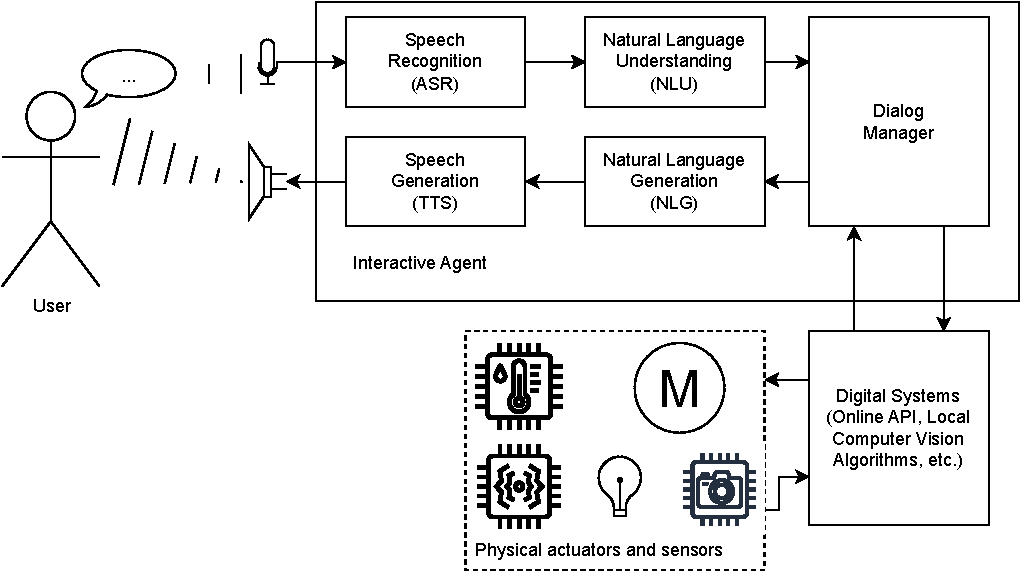
\includegraphics[width=\linewidth]{figures/schematics-generic_architecture.drawio.pdf}
  \Description{A typical interactive agent or conversational AI architecture which is interfaced a microphone and a speaker. The main system is composed of a speech recognition module, a natural language understanding module, a dialogue management module, a natural language generation module, and a speech synthesis module. It can be interfaced with the physical world through digital systems.}
  \caption{Generic architecture of a conversational interface\cite{lugrinHandbookSociallyInteractive2021}.\label{fig:architecture_conversational_interface}}
\end{figure}

\subsubsection{Natural language processing techniques}
Former techniques involved the use of a rule based system. These systems use a grammar to parse the user's input and then produce the appropriate response. The grammar is usually handcrafted, and thus the system is not really flexible (lack of robustness, and lack of scalability).

More recent NLP techniques rely on machine learning. For instance, models that are used to perform intent classification can be trained on specialized dataset (user requests as inputs and intents as outputs). This allows to roughly understand the intention of the user and in a second time to extract the entities (e.g., the location, the object, the name of a person, etc.) from the user's input. The entities and intention can then be used to perform the appropriate action.

\begin{figure}[ht]
  \centering
  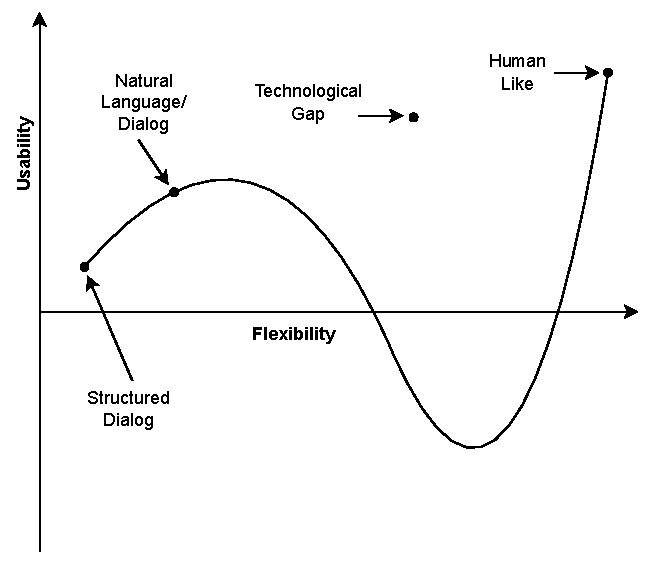
\includegraphics[width=0.7\linewidth]{figures/schematics-canny_interactive_agent.drawio}
  \caption{Approximative evolution of the usability of a spoken language interface in function of its flexibility\cite{mooreCannyApproachSpoken2019}.\label{fig:usability}}
  \Description{A theory according which the usability of an interactive agent improve to a point before decreasing again when the flexibility of the agent is being increased.}
\end{figure}

The main difficulty lay in the design of the dataset, since it is application specific and thus depends on the implemented features. Furthermore, when trying to increase the flexibility of such systems, the usability tends to decrease (see figure~\ref{fig:usability}). This may be related to the fact that increasing the flexibility is usually linked to the increase of possible user's inputs. Thus the system will be more prone to errors.

\subsubsection{Large language models}
The newest large language models are different. They can be considered as autocorrect/autofill models on steroid. They are alone \textit{only} able to predict the likeliest next words. Using them as conversational agent is in some sense a hack. It may require to fine-tune the model for this specific task (e.g., ChatGPT uses/used gpt-3.5-turbo a model fine-tuned via reinforcement learning especially for conversational tasks\cite{ouyangTrainingLanguageModels2022}). Before, it was already possible to use a few-shot technique to make GPT-3 act as a conversational AI. The idea is to provide a few examples of conversation to the model, and to let it \textit{learn} from them. This is a powerful technique that has been named \textit{prompt engineering} and is still used with ChatGPT. The given prompt provides some context to the model and will make it reply in a predictable, defined manner (e.g., it could be asked to the model to take the role of a specialized assistant for visually impaired people).

As for previous NLP techniques, large language models are able to extract the intent and entities from the user's input\cite{dunnStructuredInformationExtraction2022}. Furthermore, they can directly generate the appropriate function code to trigger some task if the prompt is well-designed.

\subsubsection{Hybrid approach}
Another approach would be a hybrid system with a more classic deep learning approach to first handle the user input. Then, if the input is too complex, pass the input to a large language model to generate the appropriate response. The main advantage of the method is that the system is more robust to exotic input and more efficient than a pure large language model. The main drawback is that it requires to train neural networks for each language and task. However, the large language model can help to train the neural network (e.g., by assisting the data mining for the dataset). The hybrid approach can help to create a working Wizard of Oz\cite{lugrinHandbookSociallyInteractive2021} with the large language model, which will facilitate the design of specialized datasets.

Remains the implementation of a prototype, which can easily be achieved using Python's modules like Flask, pyttsx3 and some APIs, like the one of OpenAI, BLOOM\cite{workshopBLOOM176BParameterOpenAccess2023} or BLOOMZ. A screenshot of the prototype's interface is shown in figure~\ref{fig:chatbot_interface}.

\begin{figure}[ht]
  \centering
  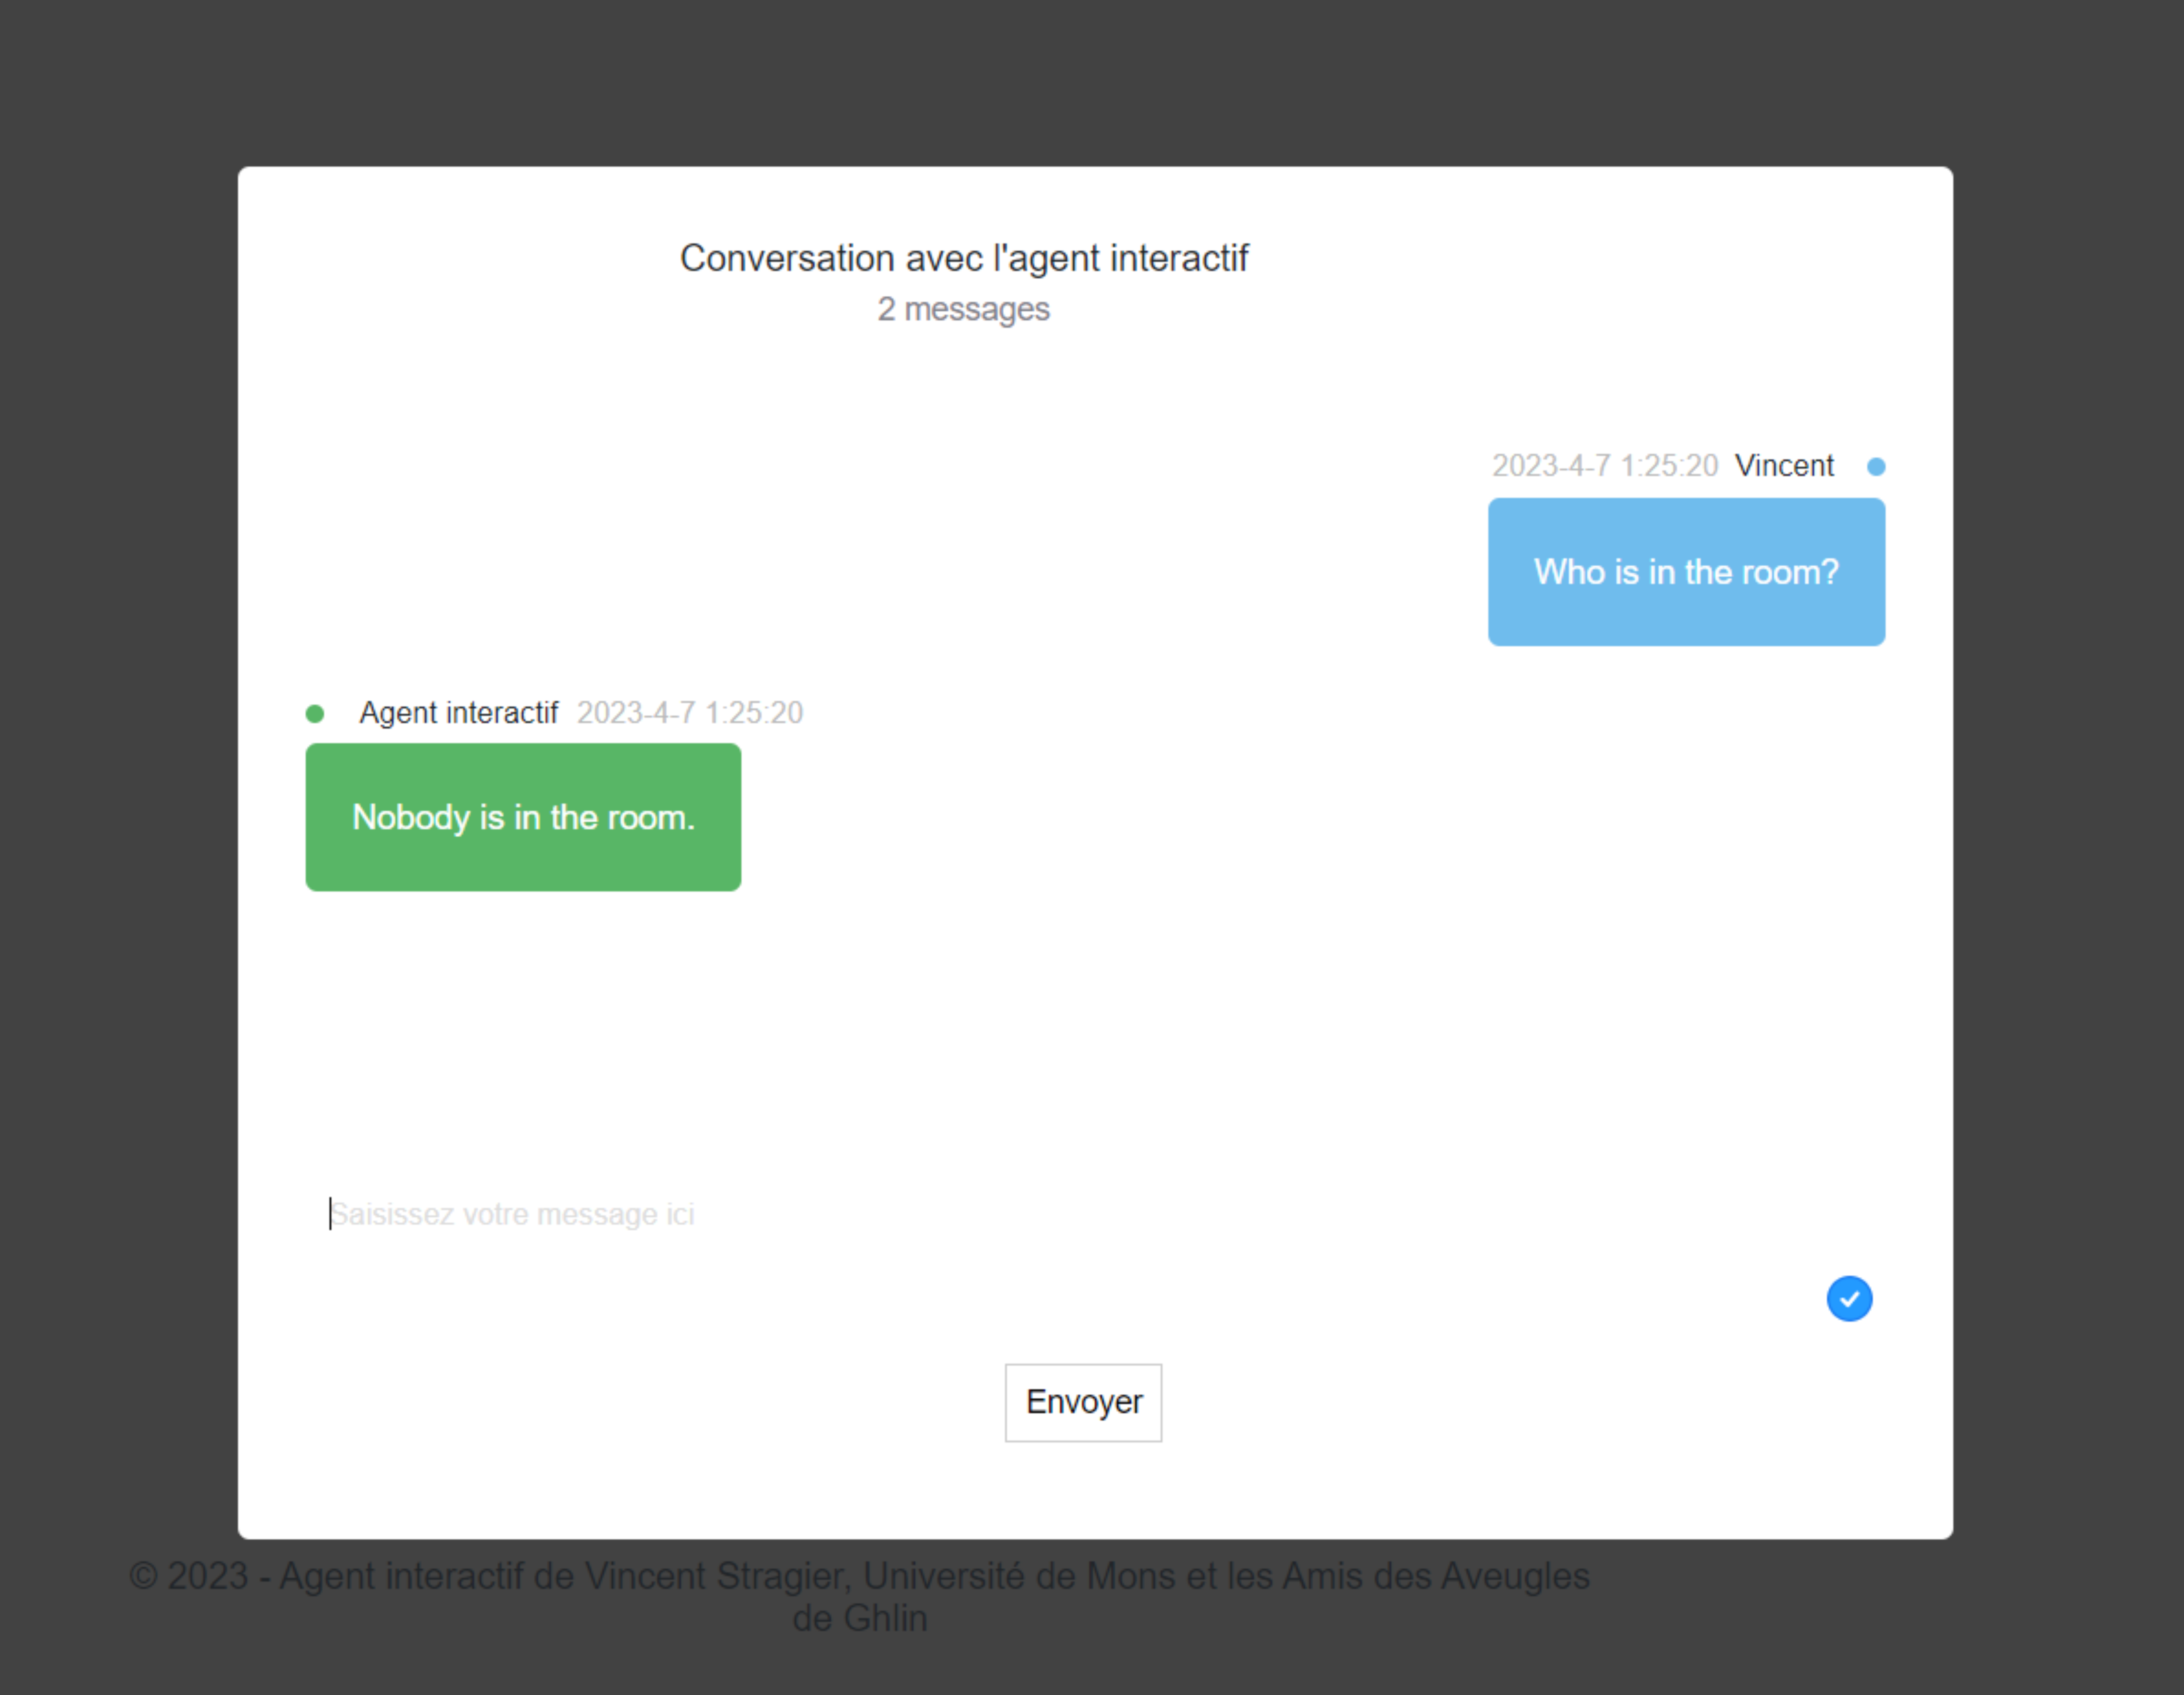
\includegraphics[width=0.7\linewidth]{figures/chatbot_interface.png}
  \caption{A screenshot of the prototype's interface.\label{fig:chatbot_interface}}
  \Description{The interface of the interactive agent prototype is accessible via a web browser. The interface is composed of a text input and a text output, with a button to send the input to the agent.}
\end{figure}

On the technical side, the current prototype is a web app connected to a web server (which can run locally) and that calls the API of the large language model (BLOOMZ in this case). The particularity of BLOOMZ is that it runs on an open source distributed system (Petals). The figure~\ref{fig:abstractive_view_interface} below shows the architecture of the prototype.

\begin{figure}[ht]
  \centering
  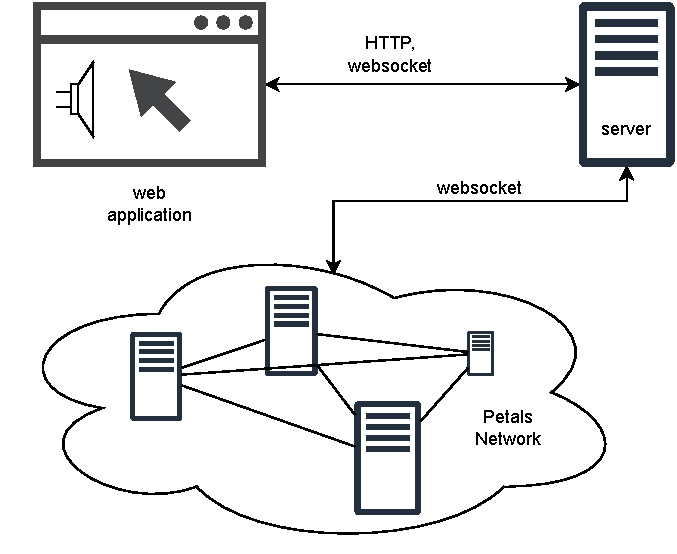
\includegraphics[width=0.5\linewidth]{figures/schematics-interactive_agent.drawio.pdf}
  \caption{Abstractive technical view of the prototype.\label{fig:abstractive_view_interface}}
  \Description{The prototype of interactive agent is composed of a web app, a web server and a large language model. The web app is connected to the web server, which is connected to the large language model (here, the Petals Network is used).}
\end{figure}

In the current state, the interface is not functional, since no module is implemented to handle the user's inputs. At the time, the reply is mocked.
% \newpage

\subsection{Prototype of facial recognition}

Being able to recognize faces is socially important (e.g., to initiate a conversation). The current state of facial recognition allows recognizing faces in real time.

The first technique of facial recognition required to manually annotate specific features on the faces, then a computer was used to compute the distances between some features and compare them between faces\cite{virgilpetrescuFaceRecognitionBiometric2019}. Later, the annotation of facial features was automated, but the reliability of the system was variable\cite{kanadeComputerRecognitionHuman1977}. These techniques were only working with portraits, then, PCA analysis (eigenfaces)\cite{pentlandFaceRecognitionUsing}, allowed to detect faces.

As shown in the previous paragraph, face detection is needed to perform face recognition. One of the efficient techniques used was the Viola-Johns algorithm\cite{violaRobustRealTimeFace2004} around 2001. More than one decade later, neural networks are used like YOLO\cite{yangRealtimeFaceDetection2018}, RetinaFace\cite{dengRetinaFaceSinglestageDense2019}, MTCNN\cite{kaziakhmedovRealworldAttackMTCNN2019}, SSD\cite{liuSSDSingleShot2016}, Dlib\cite{sharmaFARECCNNBased2016} or MediaPipe\cite{serengilDeepFaceDetection2022}. The most accurate are RetinaFace followed by MTCNN\cite{serengilDeepface2023a}.

Nowadays, for face recognition, pretrained models are used to embed the faces in a vector space. The faces are then compared using a distance metric (e.g., cosine similarity, Euclidean distance, etc.). The distance between two faces is then used to determine if the faces are the same or not. Similarly to the face detection task, multiple models exist. The current state-of-the-art models seem to be Facenet-512 (upscaled version of Facenet-128\cite{schroffFaceNetUnifiedEmbedding2015}) and VGG-Face\cite{parkhiDeepFaceRecognition2015}.

Furthermore, as stated above, other models can be used for age, sex, ethnicity, and emotion (facial expression) estimation. Here, emotion estimation could be interesting, however, it seems to be far from being accurate (the accuracy on the train set is about 98.81 \% on the train set and 56.31 \% on the test set) as shown in table~\ref{tab:confusion_matrix_emotion}. The accuracy on the test set is not very high, but it is still better than random (14.29 \%). The model used is a CNN with 3 convolutional layers, and a fully connected neural network. The model was trained on the FER2013 dataset\cite{serengilFacialExpressionRecognition2018}. The netbook used to retrain the model is accessible via this link: \url{https://gist.github.com/Vincent-Stragier/1562c159b2e0e7cda804ce153f1a83d4}.

\begin{table}[!ht]
  \caption{Confusion matrix for facial expression recognition on FER2013\cite{serengilFacialExpressionRecognition2018}.\label{tab:confusion_matrix_emotion}}
  \begin{tabular}{@{}l|ccccccc@{}}
    \toprule
             & Angry & Disgust & Fear & Happy & Sad & Surprise & Neutral \\
    \midrule
    Angry    & 200   & 2       & 57   & 45    & 80  & 14       & 49      \\
    Disgust  & 20    & 21      & 5    & 4     & 5   & 0        & 1       \\
    Fear     & 64    & 2       & 179  & 49    & 90  & 38       & 74      \\
    Happy    & 33    & 1       & 26   & 694   & 59  & 19       & 63      \\
    Sad      & 74    & 2       & 59   & 74    & 303 & 17       & 124     \\
    Surprise & 15    & 0       & 37   & 21    & 20  & 301      & 21      \\
    Neutral  & 60    & 1       & 44   & 84    & 108 & 7        & 303     \\
    \bottomrule
  \end{tabular}
\end{table}

Implementing a facial recognition system is not trivial, because, it is needed to create some sort of database (stored, either locally or on a server). Here, it has been decided for technical reason to keep the database on the server, storing some sort of ID, multiple embeddings (depending on the used models and the number of images of the user), the faces used to compute the embeddings and the user's name. The figure~\ref{fig:facial_recognition_technical_view} shows the technical view of the prototype.

\begin{figure}[!ht]
  \centering
  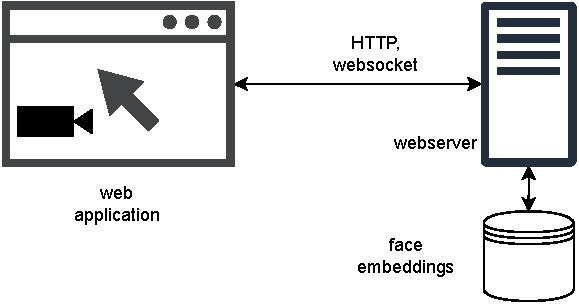
\includegraphics[width=0.7\linewidth]{figures/schematics-facial_recognition_system.drawio.pdf}
  \caption{Technical view of the prototype of facial recognition system.\label{fig:facial_recognition_technical_view}}
  \Description{The current architecture of the facial recognition system is divided in two entity. A client entity and a server entity. The client is a web application available in a browser and is used to capture images via the camera, set the various settings of the system and return the results. The server is a web server that requests the image from the client, analyse them according to the specified settings and return the results.}
\end{figure}

The current prototype allows selecting different actions, such as adding a new user (which only sends the current webcam frame to the server). It is able to detect faces using the selected model and then give an estimation of the facial expression, sex, age and ethnicity if requested. The figure~\ref{fig:facial_recognition_interface} shows a screenshot of the prototype's interface. The source code is available on GitHub at \url{https://github.com/Vincent-Stragier/webfacetools}.

\begin{figure}[!ht]
  \centering
  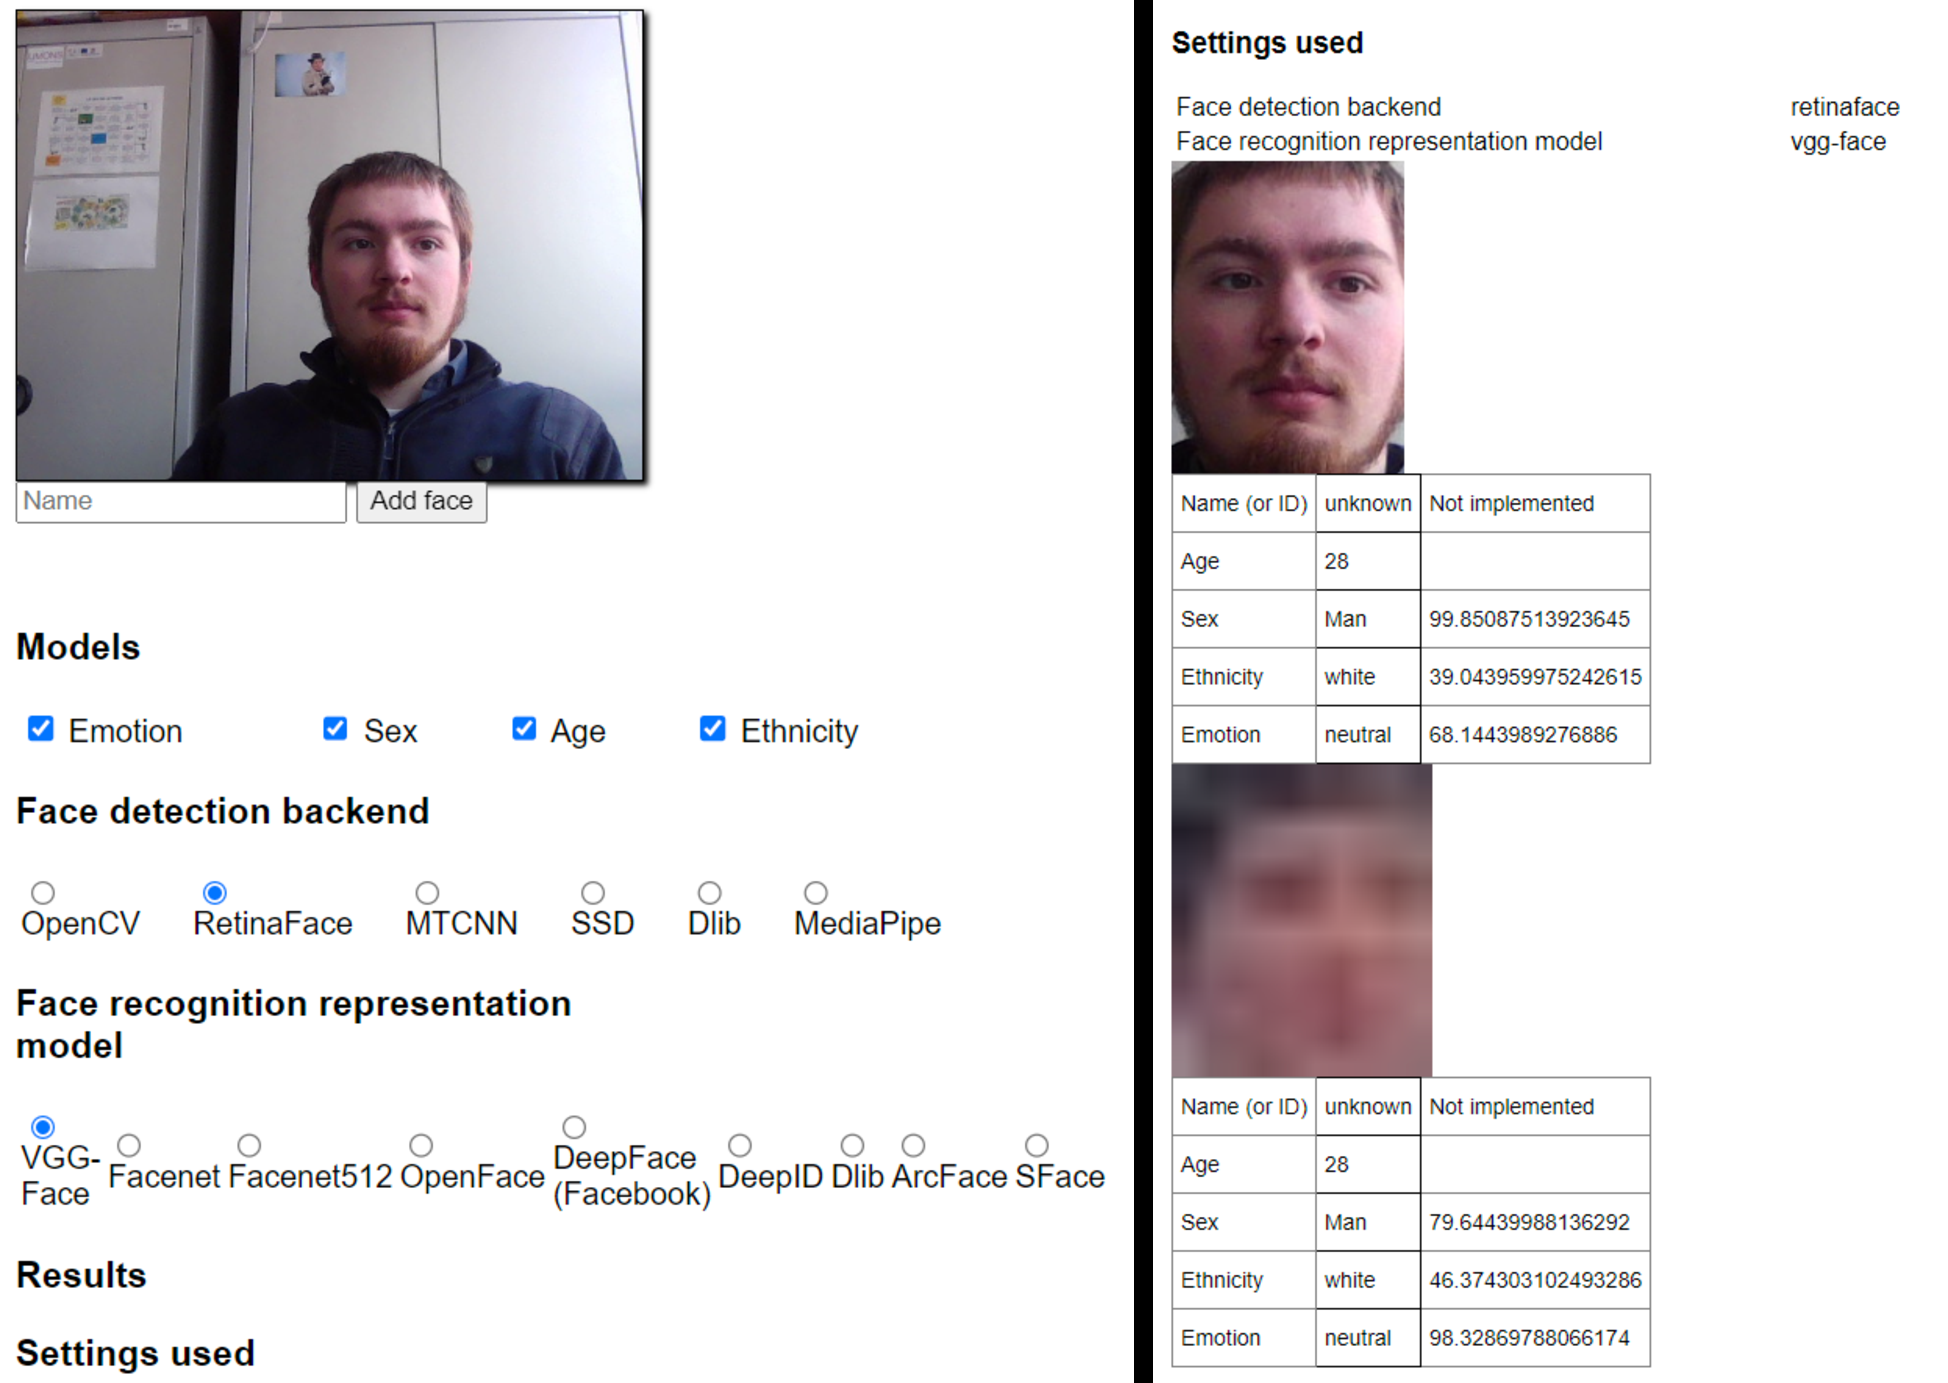
\includegraphics[width=0.65\linewidth]{figures/proto_interface.pdf}
  \caption{Two screenshots of the prototype's interface. On the left side, a live view of the camera is showed and various settings are available. On the right, two persons have been detected, and the interface shows the results of all the selected models.\label{fig:facial_recognition_interface}}
  \Description{The interface of the prototype of facial recognition system is divided in three sections. First a live view of the camera. Second, a list of settings. Third, the results of the models.}
\end{figure}
\newpage

\section{Conclusion}
The current state of the technologies shows that building a working interactive assistant is possible. The work of OpenAI and Be My Eyes is a good example of the potential of the technology. However, the current large language models are not the best fit for such a task, since they are power angry and sometime completely instable. Granted, they could be used to build less flexible but more reliable systems using current spoken language understanding systems. Eventually, open sourcing such a system could help to improve the current state of assistive technologies.

\section{Future work}
In the next years, the goal is to continue to build a prototype of an interactive assistant for blind and visually impaired people. The prototype will be improved using the technologies described above. The prototype will be tested with blind and visually impaired people to evaluate the usefulness of the prototype. It will be open sourced to allow other people to improve it. Also, a special focus will be made on open source large language models like BLOOMZ or LLaMA.

% \section{Acknowledgments}

\begin{acks}
  This research is funded by the European Regional Development Fund (ERDF). Vincent Stragier is funded through a PhD grant from the Œuvre fédérale Les Amis des Aveugles et Malvoyants ASBL- The Friends of the Blind and Visually Impaired Federal Charity-, Ghlin, Belgium.
\end{acks}

% %% the bibliography file.
\bibliographystyle{ACM-Reference-Format}
\bibliography{thesis_sources}

\end{document}
\endinput
